\newacronym{tclab}{TCLab}{\textit{Temperature Control Lab}}
\newacronym{byu}{BYU}{\textit{Brigham Young University}}
\newacronym{ncsu}{NCSU}{\textit{North Carolina State University}}
\newacronym{si}{SI}{Sistema Internacional de Unidades}

\chapter{Planta piloto}
\label{ch:planta_piloto}

O sistema experimental usado para o projeto de ações de controle é uma mini planta piloto chamada \acrlong{tclab}
(do inglês, Laboratório de Controle de Temperatura), ou apenas \acrshort{tclab}\footnote{                       % footnote
    Maiores informações sobre o \acrshort{tclab} podem ser encontrados em \href{http://apmonitor.com/heat.htm}{http://apmonitor.com/heat.htm}.
}. Esta planta foi desenvolvida na \acrlong{byu} (\acrshort{byu}) e apresentada pela primeira vez no
\textit{2017 ASEE Summer School}, na \acrlong{ncsu} (\acrshort{ncsu}). Foi desenvolvida com o
propósito de facilitar o acesso de estudantes a um laboratório de testes de controle.

Esta mini planta é essencialmente um \textit{shield} para Arduino\footnote{
    Arduino é uma plataforma de prototipagem eletrônica de hardware livre e de placa única, projetada com um    % footnote
    microcontrolador Atmel AVR com suporte de entrada/saída embutido.                                           % footnote
} contendo 2 aquecedores e 2 sensores de temperatura, mostrado na \cref{fig:tclab}. A energia dos aquecedores é
transferida através de condução, convecção e radiação até os sensores de temperatura. Tanto o controle da
potência dos aquecedores quanto as medições realizadas pelos sensores são efetuados através do Arduino.

O \acrshort{tclab} possibilita fazer a programação do controle da mini planta utilizando linguagem Python,
\acrshort{matlab} ou Simulink.

\begin{figure}[h]
	\caption{Laboratório de Controle de Temperatura}
	\begin{center}
		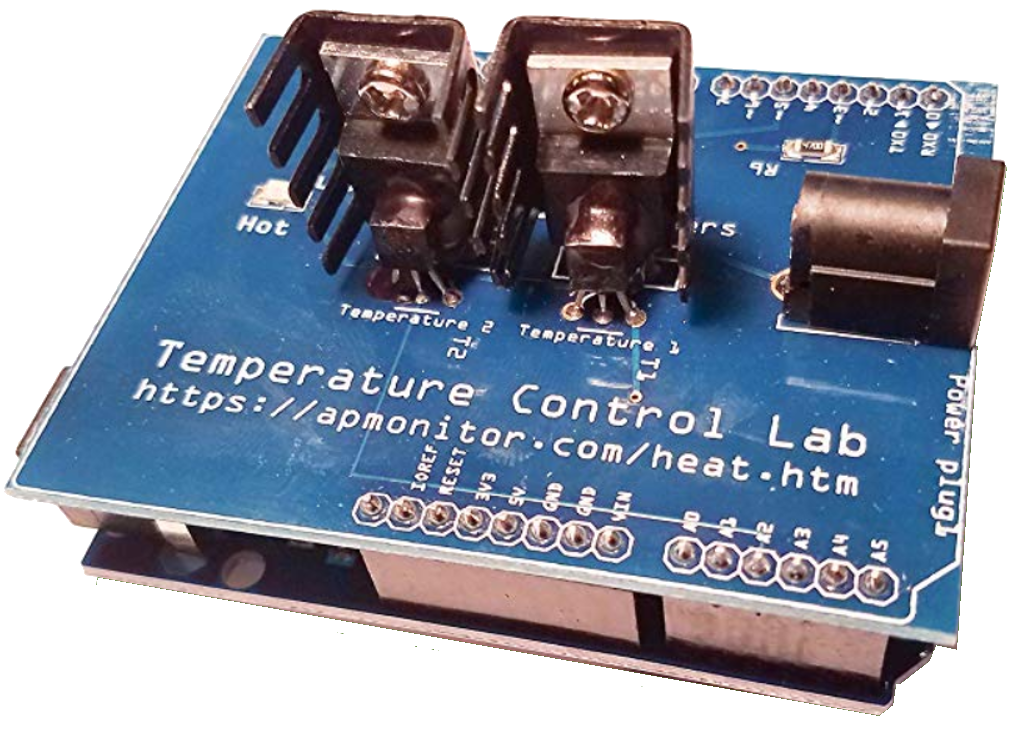
\includegraphics[width=0.55\textwidth]{./5_images/tclab.png} 
		\label{fig:tclab}
	\end{center}
	\centering
	\makebox[\width]{Fonte: ?????}  % TODO Corrigir autor
\end{figure}

% =====================================================================================================
% ============================================= Section ===============================================
% =====================================================================================================
\section{Modelagem da planta piloto}
\label{sec:modelagem_da_planta_piloto}

A modelagem teórica de balanço energético desta planta piloto é fornecida pela equipe responsável
pelo \acrshort{tclab}. São fornecidos dois modelos distintos: um para o uso de apenas um aquecedor e
um sensor, sendo assim um sistema de apenas uma entrada e uma saída, ou seja, um sistema \acrshort{siso}
(do inglês \acrlong{siso}), e outro utilizando ambos os aquecedores e sensores condidos na planta,
onde devido a proximidade existe a interferência de um no outro, sendo assim um sistema \acrshort{mimo}.
Ambos os modelos teóricos são apresentados nas seções \ref{subsec:tclab_modelo_siso} e
\ref{subsec:tclab_modelo_mimo} a seguir.

% .....................................................................................................
% ............................................ Subsection .............................................
% .....................................................................................................
\subsection{Modelo \acrshort{siso}}
\label{subsec:tclab_modelo_siso}

Segundo a equipe de desenvolvimento do \acrshort{tclab}, para a utilização de apenas um aquecedor e
um sensor é possível utilizar a \cref{eq:tclab_modelo_siso}, sendo que, para isso, deve-se assumir
que: o aquecedor e o sensor de temperatura estão na mesma temperatura; que o efeito da condução de calor
é desprezado e que as únicas trocas de calor acontecem através de radiação ou convecção; que o
aquecedor inicialmente está desligado e que tanto o aquecedor quanto o sensor inicialmente estão
em temperatura ambiente.

\begin{equation}
	\label{eq:tclab_modelo_siso}
	mC_p \dfrac{dT}{dt} = UA (T_{\infty} - T) + \epsilon \sigma A (T_{\infty}^{4} - T^{4}) + Q
\end{equation}

A \cref{tab:tclab_modelo_siso_valores} indica a descrição de cada uma das siglas da
\cref{eq:tclab_modelo_siso} e também apresenta o valor de cada um.

\begin{table}[h]
	\centering
	\caption{Valores para modelagem \acrshort{siso} do \acrshort{tclab}}
	\label{tab:tclab_modelo_siso_valores}
	\begin{tabular}{cccc} \toprule
		{Sigla} 		& {Descrição} 								& {Valor} 											& {Valor (\acrshort{si})} 							\\ \midrule
		$T_{0}$ 		& Temperatura inicial 						& $23^\circ C$ 										& $296{,}15 K $										\\
		$T_{\infty}$	& Temperatura ambiente						& $23^\circ C$										& $296{,}15 K $										\\
		$Q$				& Saída do aquecedor						& $0$ à $3 W$										& $0$ à $3 W$										\\
		$C_p$			& Capacidade de aquecimento					& $500$ $\sfrac{J}{kg.K}$							& $500$ $\sfrac{J}{kg.K}$							\\
		$A$				& Área de superfície						& $12 cm^{2}$										& $1{,}2{\times}10^{-3} m^{2}$						\\
		$m$				& Massa										& $4 g$												& $0{,}004 kg	$									\\
		$U$				& Coeficiênte global de transf. de calor	& $10$ $\sfrac{W}{m^{2}K}$							& $10$ $\sfrac{W}{m^{2}K}$							\\
		$\epsilon$		& Emissividade								& $0{,}9$											& $0{,}9$											\\
		$\sigma$		& Constante de Stefan Boltzmann				& $5{,}67{\times}10^{-8}$ $\sfrac{W}{m^{2}K^{4}}$	& $5{,}67{\times}10^{-8}$ $\sfrac{W}{m^{2}K^{4}}$	\\ \bottomrule
	\end{tabular}
\end{table}

% .....................................................................................................
% ............................................ Subsection .............................................
% .....................................................................................................
\subsection{Modelo \acrshort{mimo}}
\label{subsec:tclab_modelo_mimo}

As \cref{eq:tclab_modelo_mimo_a,eq:tclab_modelo_mimo_b} apresentam os modelos
para um sistema \acrshort{mimo}, onde ambos os aquecedores e sensores são utilizados.
As mesmas premissas descritas para o modelo \acrshort{siso} na seção \ref{subsec:tclab_modelo_siso}
devem ser aplicadas neste modelo.

\begin{subequations}
	\label{eq:tclab_modelo_mimo}
	\begin{gather}
		mC_p \dfrac{dT_1}{dt} = UA (T_{\infty} - T_1) + \epsilon \sigma A (T_{\infty}^{4} - T_{1}^{4}) + UA_s (T_2 - T_1) + \epsilon \sigma A_s (T_{2}^{4} - T_{1}^{4}) + Q_1		\label{eq:tclab_modelo_mimo_a} \\
		mC_p \dfrac{dT_2}{dt} = UA (T_{\infty} - T_2) + \epsilon \sigma A (T_{\infty}^{4} - T_{2}^{4}) + UA_s (T_1 - T_2) + \epsilon \sigma A_s (T_{1}^{4} - T_{2}^{4}) + Q_1		\label{eq:tclab_modelo_mimo_b}
	\end{gather}
\end{subequations}

A \cref{tab:tclab_modelo_mimo_valores} indica a descrição de cada uma das siglas das
\cref{eq:tclab_modelo_mimo_a,eq:tclab_modelo_mimo_b} e também apresenta o valor de cada um.

\begin{table}[h]
	\centering
	\caption{Valores para modelagem \acrshort{mimo} do \acrshort{tclab}}
	\label{tab:tclab_modelo_mimo_valores}
	\begin{tabular}{cccc} \toprule
		{Sigla} 		& {Descrição} 								& {Valor} 											& {Valor (\acrshort{si})} 							\\ \midrule
		$T_{0}$ 		& Temperatura inicial 						& $23^\circ C$ 										& $296{,}15 K $										\\
		$T_{\infty}$	& Temperatura ambiente						& $23^\circ C$										& $296{,}15 K $										\\
		$Q$				& Saída do aquecedor						& $0$ à $3 W$										& $0$ à $3 W$										\\
		$C_p$			& Capacidade de aquecimento					& $500$ $\sfrac{J}{kg.K}$							& $500$ $\sfrac{J}{kg.K}$							\\
		$A$				& Área de superfície						& $10 cm^{2}$										& $1{\times}10^{-3} m^{2}$							\\
		$A_s$			& Área de superfície (entre dissipadores)	& $2 cm^{2}$										& $2{\times}10^{-4} m^{2}$							\\
		$m$				& Massa										& $4 g$												& $0{,}004 kg	$									\\
		$U$				& Coeficiênte global de transf. de calor	& $10$ $\sfrac{W}{m^{2}K}$							& $10$ $\sfrac{W}{m^{2}K}$							\\
		$\epsilon$		& Emissividade								& $0{,}9$											& $0{,}9$											\\
		$\sigma$		& Constante de Stefan Boltzmann				& $5{,}67{\times}10^{-8}$ $\sfrac{W}{m^{2}K^{4}}$	& $5{,}67{\times}10^{-8}$ $\sfrac{W}{m^{2}K^{4}}$	\\ \bottomrule
	\end{tabular}
\end{table}